% Copyright 2021 Edoardo Riggio

% Licensed under the Apache License, Version 2.0 (the "License");
% you may not use this file except in compliance with the License.
% You may obtain a copy of the License at

% 	http://www.apache.org/licenses/LICENSE-2.0

% Unless required by applicable law or agreed to in writing, software
% distributed under the License is distributed on an "AS IS" BASIS,
% WITHOUT WARRANTIES OR CONDITIONS OF ANY KIND, either express or implied.
% See the License for the specific language governing permissions and
% limitations under the License.

\documentclass{article}

\usepackage{amsmath, graphicx, hyperref}
\usepackage{fancyvrb, newverbs, xcolor}

\definecolor{cverbbg}{gray}{0.93}

\newenvironment{cverbatim}
 {\SaveVerbatim{cverb}}
 {\endSaveVerbatim
  \flushleft\fboxrule=0pt\fboxsep=.5em
  \colorbox{cverbbg}{\BUseVerbatim{cverb}}%
  \endflushleft
}

\newenvironment{lcverbatim}
 {\SaveVerbatim{cverb}}
 {\endSaveVerbatim
  \flushleft\fboxrule=0pt\fboxsep=.5em
  \colorbox{cverbbg}{%
    \makebox[\dimexpr\linewidth-2\fboxsep][l]{\BUseVerbatim{cverb}}%
  }
  \endflushleft
}

\newcommand{\ctexttt}[1]{\colorbox{cverbbg}{\texttt{#1}}}
\newverbcommand{\cverb}
  {\setbox\verbbox\hbox\bgroup}
  {\egroup\colorbox{cverbbg}{\box\verbbox}}

\begin{document}
\begin{titlepage}
    \begin{center}
        \vspace*{1cm}
        
        \Huge
        \textbf{Data Management Cheatsheet}
        
        \vspace{0.5cm}
        \LARGE
        
        \vspace{.5cm}
        
        Edoardo Riggio
   		  \vspace{1.5cm}
       
        \vfill
        
        \today
        
        \vspace{.8cm}
          \Large
          Computer Networking - SP. 2021 \\
        Computer Science\\
        Universit\`{a} della Svizzera Italiana, Lugano\\
        
    \end{center}
\end{titlepage}

\tableofcontents

\newpage

\section{Entity Relationship Models}
\subsection{Purpose}
Provides a common, informal, and convenient method for communication between application end users and the database designers in order to model the information's structure. \\ \\
The ER model frequently employs \textbf{ER diagrams}, which are pictorial descriptions to visualize the information's structure.

\subsection{Basic Concepts}
The three basic concepts are:
\subsubsection{Entity}
It is an "object". All entities of the same "type" form an \textbf{entity set}. \\ \\
Pictorially, it is denoted by a rectangle, with its type written inside. It must be a singular noun and capitalized (all capitals for acronyms). \\ \\

\centerline{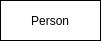
\includegraphics[width=2cm]{./assets/entity.png}}
	
\subsubsection{Attribute}
An entity can have a set of zero or more attributes, which are some properties. All entities in the entity set has the same set of properties, though not generally with the same values. \\ \\
Pictorially, attributes of an entity are written in ellipses connected to the entity. \\ \\ \\

\centerline{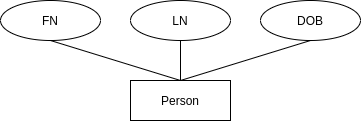
\includegraphics[width=7.5cm]{./assets/attribute.png}}
\vspace{.6cm}
Attributes can be of several different types:

\begin{itemize}
	\item \textbf{Base}
	
	\item \textbf{Simple}
	
	\item \textbf{Single-valued}
	
	\item \textbf{Derived}
	\vspace{.2cm} \\
	An attribute which value is derived from other factors (e.g. age from DOB and the current date). \\ \\
	
	\centerline{
\includegraphics[width=2cm]{./assets/derived.png}}
	
	\item \textbf{Composite}
	\vspace{.2cm} \\
	An attribute that has multiple component attributes attached to it. \\ \\
	
	\centerline{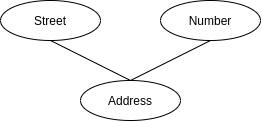
\includegraphics[width=5.2cm]{./assets/composite.png}}
	
	\item \textbf{Multi-valued}
	\vspace{.2cm} \\
	Unspecified number of values in this type of attribute. \\ \\
	
	\centerline{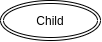
\includegraphics[width=2cm]{./assets/multivalued.png}}
\end{itemize}
	
\subsubsection{Relationship}
Several entity sets can participate in a relationship.\\ \\
Pictorially, a relationship is defined as a diamond with a verb inside. This verb should be in third person singular and capitalized. \\ \\
Relationships can be:

\begin{itemize}
	\item \textbf{Binary}
	\vspace{.2cm} \\
	A binary relationship can be \textbf{many-to-one} iff for each element of A there exists at most one element of B related to it (e.g. the relationship "born" between a person and a country). \\ \\
	
	\centerline{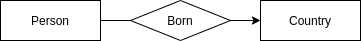
\includegraphics[width=7cm]{./assets/many-to-one.png}}
	\vspace{.6cm}
	A binary relationship can be \textbf{one-to-one} iff for each element of A there exists at most one element of B related to it, and for each element of B there exists at most one element of A related to it (e.g. the relationship "heads" between a person and a country). \\ \\
	
	\centerline{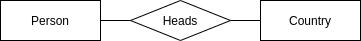
\includegraphics[width=7cm]{./assets/one-to-one.png}}
	\vspace{.6cm}
	A binary relationship can be \textbf{many-to-many} if it is not many-to-one from A to B, and it is not many-to-one from B to A (e.g. the relationship "likes" between a person and a country). \\ \\
	
	\centerline{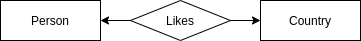
\includegraphics[width=7cm]{./assets/many-to-many.png}}
	\vspace{.6cm}
	
	\item \textbf{Ternary}
	\vspace{.2cm} \\
	This relationship is between three distinct entity relationship. \\ \\
	
	\centerline{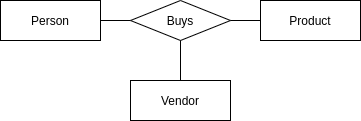
\includegraphics[width=7cm]{./assets/ternary.png}}
	\vspace{.6cm}
	
	\item \textbf{Non-Distinct Entity Set}
	\vspace{.2cm} \\
	Frequently in this case is useful to gives roles to the participating entities. \\ \\
	
	\centerline{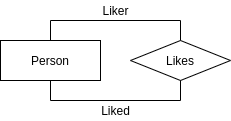
\includegraphics[width=4.5cm]{./assets/nondistinct.png}}
	\vspace{.6cm}
\end{itemize}

\subsection{Keys}
Some subset of the attributes of an entity has the property that two different entities in an entity set must \textbf{differ on the values of the attributes}. Such a set of attributes is called a \textbf{superkey}. A minimal superkey is called a \textbf{key}.

\subsubsection{Primary Keys}
If an entity as one or more keys, then one of them is chosen as the \textbf{primary key}. \\ \\

\centerline{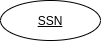
\includegraphics[width=2cm]{./assets/key.png}}

\subsection{Relationships as Entities}
By considering relationships as entities, it allows us to let relationships participate in other "high order" relationships. \\ \\ \\

\centerline{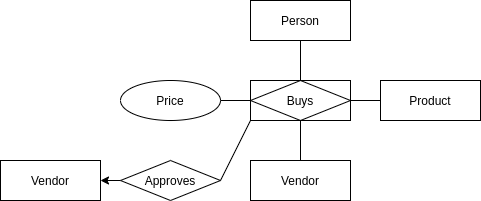
\includegraphics[width=9cm]{./assets/rel-ent.png}}
\vspace{.6cm}

\subsection{Strong and Weak Entities}
The elements of a \textbf{strong entity set} can be identified by the values of their attributes. That is, it has a primary key made of its attributes. \\ \\
The elements of a \textbf{weak entity set} cannot be identified by the values of their attributes. There is no primary key made from its own attributes. \\ \\
In the case below, a Man can only be identified by the combination of: the Woman to whom he is related, and his Name -- which is now a \textbf{discriminant}. \\ \\ \\

\centerline{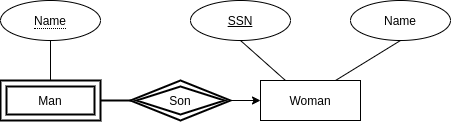
\includegraphics[width=8cm]{./assets/weak.png}}
\vspace{.6cm}

\subsection{ISA Relationships}
The subset relationship between the set and its subset is called ISA. The elements of the subset all have the same attributes and relationships as the elements of the set. In addition, they may participate in relationships and have attributes that make sense for them. \\ \\
The elements of the subset are \textbf{weak entities}. \\ \\ \\

\centerline{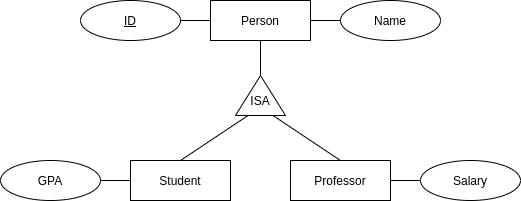
\includegraphics[width=9.5cm]{./assets/isa.png}}
\vspace{.6cm}

\begin{itemize}
	\item \textbf{Disjoint}
	\vspace{.2cm} \\
	No Entity could be in more than one subclass.
	
	\item \textbf{Overlapping}
	\vspace{.2cm} \\
	An Entity could be in more than one subclass.
	
	\item \textbf{Total}
	\vspace{.2cm} \\
	Every Entity has to be in at least one subclass.
	
	\item \textbf{Partial}
	\vspace{.2cm} \\
	An Entity does not have to be in any subclass.
\end{itemize}

\subsection{Cardinality Constraints}
It is possible to specify how many times each entity from some entity set can participate in some relationship. Constraint can be specified as:

\begin{itemize}
	\item \textbf{0..*}
	\vspace{.2cm} \\
	Means there are no constraints.
	
	\item \textbf{i..i}
	\vspace{.2cm} \\
	Means that the constraint must be exactly $i$.
	
	\item \textbf{i..j}
	\vspace{.2cm} \\
	Means that the constraints can go from $i$ up to $j$.
\end{itemize}
Constraints are \textbf{look across}, meaning that in the following example:

\begin{itemize}
	\item Every person likes exactly 1 country
	\item Every country is liked by 2 or 3 people
\end{itemize}

\vspace{.6cm}
\centerline{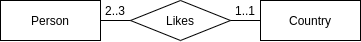
\includegraphics[width=7cm]{./assets/look-across.png}}
\vspace{.2cm}

\section{Relational Model}
\subsection{Sets}
A set is a "bag" of elements, some or all of which could be sets themselves. It is not possible to specify \textbf{how many times} or \textbf{in which position} does an element appear in a set.

\subsection{Relations}
Relations are elements such as \textbf{primary keys}, \textbf{keys}, \textbf{foreign keys}...

\subsubsection{Keys and Superkeys}
A set of columns in a relation is a \textbf{superkey} iff any two tuples that are equal on the elements of these columns are completely equal. A relation has always \textbf{at least one} superkey. The set of all the attributes is a superkey. \\ \\
A minimal superkey is a \textbf{key}. A relation always has at least one key (but there could be more than one). Exactly one key is chosen to as the \textbf{primary key}.

\subsubsection{Foreign Keys}
A foreign key is a column or group of columns in a relational database table that provides a link between data in two tables. It must always reference to a primary key somewhere in the database.

\subsection{Crow's Feet}
Crows Feet are used to indicate constraint. The following are the possible Crow's Feet: \\ \\

\centerline{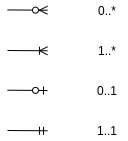
\includegraphics[width=3cm]{./assets/crows.png}}


\end{document}

























